% ============================================================
% Lampiran pengajuan ISBN — lintas OS (cukup TeX, tanpa alat lain)
% Isi: halaman 2 s.d. sebelum BAB 1 dari main.pdf
% (halaman judul, halaman redaksi, prakata, daftar isi).
%
% Cara pakai (Windows/macOS/Linux):
%   1) kompilasi buku : latexmk -pdf main
%   2) kompilasi ini  : pdflatex lampiran-isbn
% Batas halaman dibaca otomatis dari lampiran-batas.txt yang ditulis
% bukupedia.cls saat \mainmatter. (Pengguna Linux/macOS bisa juga
% memakai "make lampiran".)
% ============================================================
\documentclass{article}
\usepackage[paperwidth=15.5cm, paperheight=23cm, margin=0cm]{geometry}
\usepackage{pdfpages}
\begin{document}
\IfFileExists{lampiran-batas.txt}{}{%
  \errmessage{lampiran-batas.txt tidak ditemukan - kompilasi dulu
    main.tex dengan bukupedia.cls terbaru (latexmk -pdf main)}}
\newread\bkpbatas
\openin\bkpbatas=lampiran-batas.txt
\read\bkpbatas to \bkpakhir
\closein\bkpbatas
\includepdf[pages={2-\bkpakhir}]{main.pdf}
\end{document}
